\documentclass{article}

\usepackage[spanish]{babel}
\usepackage{mathdots}
\usepackage{listings}
\usepackage{color}
\usepackage[numbers,sort&compress]{natbib}
\usepackage{graphicx}
\usepackage{subfigure}
\usepackage{url}
\usepackage{amsmath}
\usepackage{hyperref}
\usepackage[top=15mm, bottom=40mm, left=15mm, right=15mm]{geometry}
\setlength{\parskip}{2mm}
\setlength{\parindent}{0pt}

\setlength{\parskip}{2mm}
\setlength{\parindent}{0pt}
\definecolor{blue}{rgb}{0,0.6,0}
\definecolor{gray}{rgb}{0.3,0.3,0.3}
\definecolor{orange}{rgb}{0.8,0.4,0}
\definecolor{mostaza}{rgb}{0.9,0.8,0.1}

\lstset{ %
  language=R,                     % the language of the code
  basicstyle=\footnotesize,       % the size of the fonts that are used for the code
  numbers=left,                   % where to put the line-numbers
  numberstyle=\tiny\color{gray},  % the style that is used for the line-numbers
  stepnumber=1,                   % the step between two line-numbers. If it's 1, each line
                                  % will be numbered
  numbersep=5pt,                  % how far the line-numbers are from the code
  backgroundcolor=\color{white},  % choose the background color. You must add \usepackage{color}
  showspaces=false,               % show spaces adding particular underscores
  showstringspaces=false,         % underline spaces within strings
  showtabs=false,                 % show tabs within strings adding particular underscores
  frame=single,                   % adds a frame around the code
  rulecolor=\color{black},        % if not set, the frame-color may be changed on line-breaks within not-black text (e.g. commens (green here))
  tabsize=2,                      % sets default tabsize to 2 spaces
  captionpos=b,                   % sets the caption-position to bottom
  breaklines=true,                % sets automatic line breaking
  breakatwhitespace=false,        % sets if automatic breaks should only happen at whitespace
  title=\lstname,                 % show the filename of files included with \lstinputlisting;
                                  % also try caption instead of title
  keywordstyle=\color{orange},      % keyword style
  commentstyle=\color{blue},   % comment style
  stringstyle=\color{mostaza},      % string literal style
  escapeinside={\%*}{*)},         % if you want to add a comment within your code
  morekeywords={*,...}            % if you want to add more keywords to the set
} 

\author{1445183}
\title{Práctica 10: algoritmo genético}
\date{\today}

\begin{document}

\maketitle

\section{Objetivo}
Estudiar los efectos del tiempo de ejecución del código paralelizado proporcionado por la práctica \cite{elisaweb10} variando el número de objetos en las tres instancias siguientes: \par
\textit{1.-} El peso y el valor de cada objeto se generan independientemente con una distribución normal \par
\textit{2.-} El peso de cada objeto se generan independientemente con una distribución normal y su valor es correlacionado con el peso, con un ruido normalmente distribuido de baja magnitud \par
\textit{3.-} El peso de cada objeto se generan independientemente con una distribución normal y su valor es inversamente correlacionado con el peso, con un ruido normalmente distribuido de baja magnitud

\section{Descripción}

El código se paraleliza desde el principio, usando tres núcleos de los cuatro posibles

\begin{lstlisting}[language=R]
library(testit)
suppressMessages(library(doParallel))
cls <- makeCluster(detectCores() - 1)
registerDoParallel(cls)
\end{lstlisting}

Se paralelizan las funciones de mutación, reproducción, factibilidad y objetivo basado en el código de \textit{Reyna Fernández} \cite{yess10}
\begin{lstlisting}[language=R]
mutacion2<- function() { 
  if (runif(1) < pm) {
    return(mutacion(p[i,], n))
  }
}

reproduccion2<- function() {
  padres <- sample(1:tam, 2, replace=FALSE)
  hijos_t <- reproduccion(p[padres[1],], p[padres[2],], n)
  return(hijos_t)
}

objetivo2<- function() {
  obj_t <- double()
  obj_t <- c(obj_t, objetivo(p[i,], valores))
  return(obj_t)
}

factible2 <- function() {
  fact_f <- integer()
  fact_f <- c(fact_f, factible(p[i,], pesos, capacidad))
  return(fact_f)
  
}

\end{lstlisting}

después se dan las indicaciones que se piden en el \textit{objetivo} en relación \textit{peso} y \textit{valor} y se varía el número de objetos por instancia con valores de \texttt{30, 50} y \texttt{80}, se toma el tiempo de ejecución usando \texttt{system.time}

\begin{lstlisting}[language=R]
n <- seq(30,50,80)
for(ins in 1:3) {
  
  if(ins == 1) {
    valores <- generador.valores(pesos, 10, 500)
  } else if(ins == 2) {
    valores <- generador.valores.correlacionados(pesos,10,500)
  } else if(ins == 3) {
    valores <- generador.valores.correlacionados(rev(pesos),10,500)
  }
\end{lstlisting}

\newpage


\section{Resultados}
En la figura \ref{fig2} se puede observar el tiempo que se tarda en dar 50 pasos, los colores corresponden a las instancias indicadas anteriormente. \par 
El tiempo es aumenta cuando se tiene correlación y la cantidad de onjetos aumenta, cuando la correlación es inversa se tarda menos tiempo conforme se tiene más cantidad de objetos y cuando los valores son independientes, es decir, no están correlacionados no se tiene una secuencia fija en el tiempo al cambiar la cantidad de objetos. \par 
Línea negra - sin correlación \par
\textcolor{green}{Línea verde} - correlación \par
\textcolor{blue}Línea morada - correlación inversa

\begin{figure}[h!]
\centering
\subfigure[30 objetos]{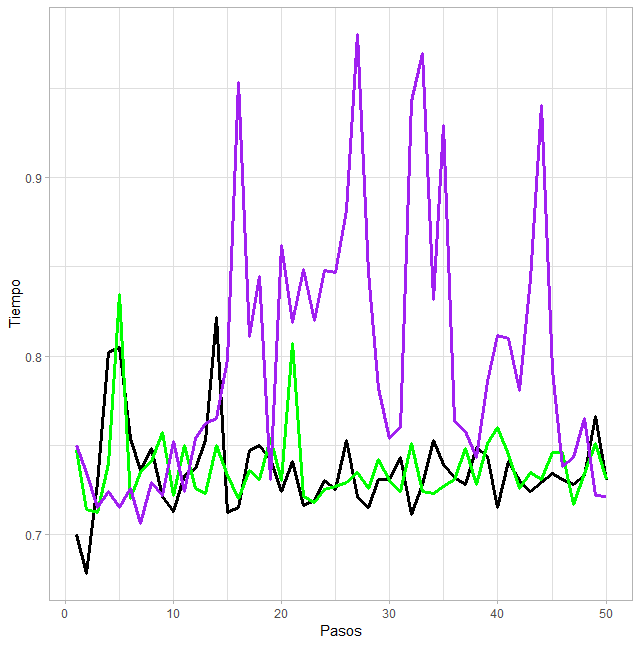
\includegraphics[width=60mm]{./image30.png}}
\subfigure[50 objetos ]{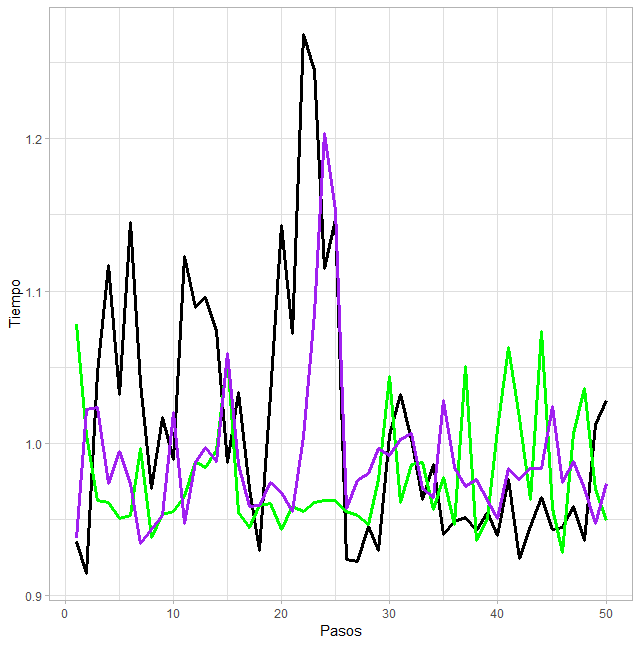
\includegraphics[width=60mm]{./image50.png}}
\subfigure[80 objetos]{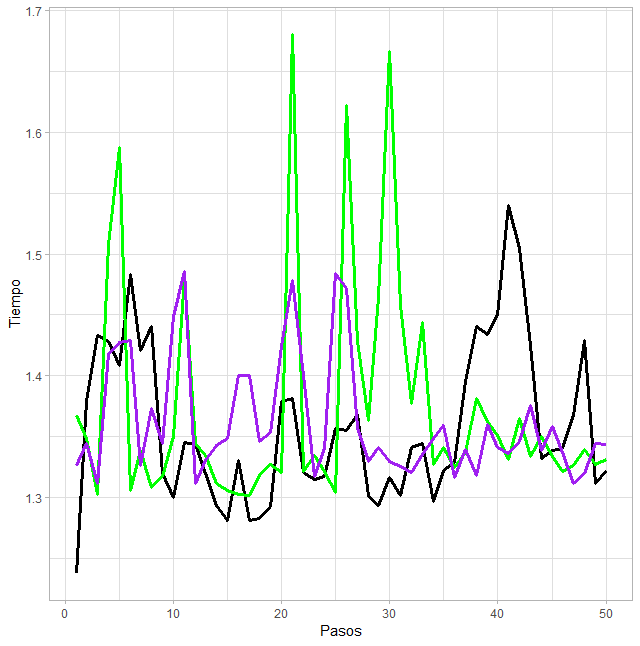
\includegraphics[width=60mm]{./image80.png}}
\caption{Interacción de partículas}\label{fig2}
\end{figure}






\newpage
\section{Conclusión}

Es más fácil (rápido) decidir por objetos  que valen mucho y pesan poco como pasa en la correlación inversa, donde el tiempo es menor. \par
Que los objetos pesen más pero tengan poco valor, hace que tarde en decidir si llevarlos o no, como pasa en la correlación.


\newpage
\bibliographystyle{plainnat}
\bibliography{bibliosimu}

\end{document}